\documentclass[12pt]{article}

\input{~/Desktop/LosDelDGIIM.github.io/subjects/_assets/preambulo}

\author{Joaquín Avilés de la Fuente \and Arturo Olivares Martos}
\date{\today}
\title{Memoria Práctica \texttt{Lex}\\Modelos de Computación}


\lstset{
    basicstyle=\ttfamily,
    keywordstyle=\color{blue},
    stringstyle=\color{red},
    commentstyle=\color{green},
    morekeywords={00,34},
    escapeinside={(*@}{@*)}
}

\begin{document}    

    \maketitle
    \tableofcontents

    \begin{abstract}
        En la presente memoria se detallará la práctica llevada a cabo en la asignatura de Modelos de Computación del tercer curso del Doble Grado en Ingeniería Informática y Matemáticas de la Universidad de Granada.
        En ella, hemos implementado un menú con diversas funciones para analizar un texto introducido por el usuario, el cual detallaremos más adelante en las distintas secciones de la memoria.
    \end{abstract}

    \newpage
    \section{Introducción}

    En nuestro caso, para no limitarnos a un único caso de uso, lo cual probablemente implicaría usar menos expresiones regulares, hemos decidido implementar un menú con diversas opciones que permiten al usuario analizar un texto introducido por él mismo. Esto proporciona así más versatilidad, a la vez que nos facilita la implementación de un mayor número de expresiones regulares.

    La funcionalidad del programa se puede probar de forma directa mediante el menú creado, o se puede tambiar probar por separado con cada programa. Además, hemos creado un archivo \verb|makefile| que permite que la ejecución sea más sencilla.

    Todos estos aspectos los explicaremos de forma detallada en cada una de las secciones de este artículo.

    \begin{observacion}
    Todos las rutas relativas que se proporcionan suponen que nos encontramos en la carpeta raíz de esta práctica.
    \end{observacion}

    \section{Comprobación de Números de Teléfono}

    Este analizador se encuentra en el archivo \verb|regex_tfno.l|. Para compilarlo, se debe ejecutar el siguiente comando:
    \begin{minted}[linenos=false]{shell-session}
        $ flex++ -o regex_tfno.cpp regex_tfno.l
        $ g++ -Wall -o regex_tfno regex_tfno.cpp -lfl
    \end{minted}

    Para ejecutarlo, se debe ejecutar el siguiente comando:
    \begin{minted}[linenos=false]{shell-session}
        $ ./regex_tfno <fichero>
    \end{minted}
    donde \verb|<fichero>| es el archivo que se desea analizar en busca de números de teléfono.
    De forma alternativa, se recomienda usar el \verb|makefile| proporcionado usando la siguiente regla:
    \begin{minted}[linenos=false]{shell-session}
        $ make telefonos
    \end{minted}
    En este caso, el archivo de texto que se analizará es \verb|Telefonos/telefonos.txt|, por lo que deberá almacenarse en ese archivo las cadenas que se deseen procesar.\\

    Este programa analiza el archivo pasado en búsqueda de números de teléfono. Por un lado, informa de las cadenas que no han sido identificadas con números de teléfono de ningún país registrado y, por otro lado, de los números de teléfono válidos que se han encontrado, informa en qué país son válidos. Actualmente tan solo se ha implementado la detección de números de teléfono españoles, puesto que son los que conocemos de primera mano, pero la extensión a otros países es directa.
    Para detectar los números de teléfono, se han usado las siguientes expresiones regulares:
    \begin{itemize}
        \item \ul{\texttt{tfno\_espanol\_grupos3}}:
        \begin{lstlisting}
((00|"+")34(" ")?)?([0-9]{3}(" ")?){3}
        \end{lstlisting}
        
        En este caso, se da la posibilidad a que el número de teléfono esté agrupado en grupos de 3 cifras, separados por un espacio. En primer lugar, puede comenzar con el prefijo internacional (\verb|34| en el caso de España), que ha de ir precedido de \verb|00| o \verb|+|. A continuación, se encuentras los tres grupos de 3 cifras, en total 9 cifras. Se permite que haya un espacio entre los grupos de cifras y tras el prefijo internacional.

        \item \ul{\texttt{tfno\_espanol\_grupos2}}:
        \begin{lstlisting}
((00|"+")34(" ")?)?([0-9]{3}(" ")?){1}([0-9]{2}(" ")?){3}
        \end{lstlisting}
        
        Esta expresión es similar, solo que permite que los 6 últimos finales se agrupen en tres grupos de 2 cifras, en lugar de dos grupos de 3 cifras. De nuevo, se permite que haya un espacio entre los grupos de cifras y tras el prefijo internacional (si lo hay).
    \end{itemize}

    Hemos limitado a estos casos, puesto que son los más habituales en España. No obstante, se podrían añadir más expresiones regulares para detectar otros formatos de números de teléfono. Tenemos por tanto la siguiente regla, la cual fuerza a que se cumpla una de las dos expresiones regulares anteriores, y esto sea lo único que se encuentre en la línea:
    \begin{minted}[
        fontsize=\footnotesize,
        linenos=false,
        breaklines=false
    ]
        {c++}
        ^{tfno_espanol_grupos3}|{tfno_espanol_grupos2}$   {tfno_pais["España"].insert(yytext);}
    \end{minted}
    Como vemos, los teléfonos detectados los almacenamos en un conjunto asociado a la clave \verb|España|, de forma que sería muy fácilmente generalizable a un mayor número de países. Un ejemplo de funcionamiento de este programa se encuentra en la Figura~\ref{fig:telefonos}.
    \begin{figure}
        \centering
        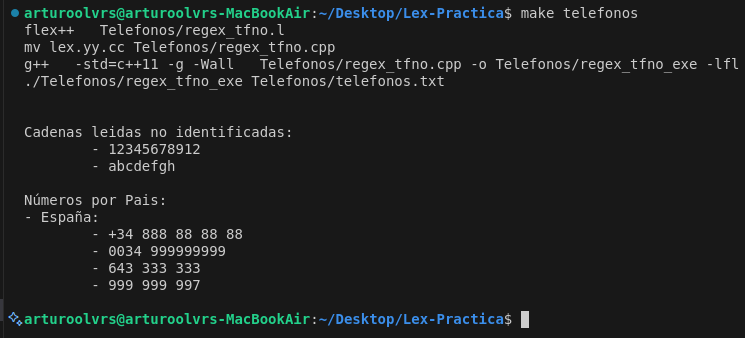
\includegraphics[width=\textwidth]{Img/Funcionamiento_Tfno.png}
        \caption{Ejemplo de ejecución del programa \texttt{regex\_tfno}.}
        \label{fig:telefonos}
    \end{figure}


\end{document}
